\documentclass{article}
\usepackage[utf8]{inputenc}
\usepackage[]{hyperref}
\usepackage{tikz}
\def\checkmark{\tikz\fill[scale=0.4](0,.35) -- (.25,0) -- (1,.7) -- (.25,.15) -- cycle;} 

\title{Milestone Report: Toxic Comment Challenge with Deep Learning NLP Techniques}
\author{Anthony Ho and Michael Baumer}
\date{\today}

\usepackage[square,sort,comma,numbers]{natbib}
\usepackage{graphicx}
\usepackage[paper=letterpaper,margin=0.75in]{geometry}

\begin{document}
\maketitle

\begin{enumerate}
    \item \textbf{Team:} Michael Baumer (mbaumer) and Anthony Ho (ahho)
    \item \textbf{Mentor:} Tim Shi
    \item \textbf{Problem Description:} Many websites with user-submitted content must deal with toxic or abusive comments, but require increasingly fine-grained comment classifications to maintain civility without interfering with normal discourse. In this project, we will improve the identification and fine-grained classification of toxic online comments (Kaggle challenge suggested on course website, online at:
    
    \url{https://www.kaggle.com/c/jigsaw-toxic-comment-classification-challenge})
    
    \item \textbf{Data:} We will be using a dataset of 159,571 comments from Wikipedia’s talk page edits which have been labeled by human raters for toxic behavior. The types of toxicity are: \texttt{toxic}, \texttt{severe\_toxic}, \texttt{obscene}, \texttt{threat}, \texttt{insult}, and \texttt{identity\_hate}. The dataset is available at the Kaggle website. 
    
    \item \textbf{Baseline Algorithm:} For our baseline algorithm, we take the average of the 300d GloVe embeddings of all words in each comment, and use this as input into a fully-connected 3-hidden-layer neural network (with 30, 20, 10 hidden units in each hidden layer respectively and ReLU activation), with a sigmoid output layer (since we are performing multi-label classification, i.e. each type of toxicity are not mutually exclusive).
    
    \item \textbf{Evaluation:} We have set up a evaluation pipeline to automatically (1) plot ROC curves or precision-recall curve for classification of each toxicity type, (2) compute the ROC AUC or average precision for classification of each toxicity type, (3) compute the mean column-wise ROC AUC or mean column-wise average precision across all toxicity types. We will be running the final test on a test set of 153,164 comments with true labels withheld by Kaggle, which will be scored according to mean column-wise ROC AUC as the official evaluation metric in the Kaggle Challenge.
    
    \item \textbf{Results:} We find relatively good dev set performance as measured by the ROC curves for each toxicity type (see Figure \ref{fig:roc}). The mean column-wise ROC AUC on the blind test set is 0.9490, which is good performance for a baseline, but places us at only \#2806 out of 3268 entries in the challenge. The similarity between the train and dev set curves shows that we are not overfitting.
    
    \begin{figure}[h]
    \centering
    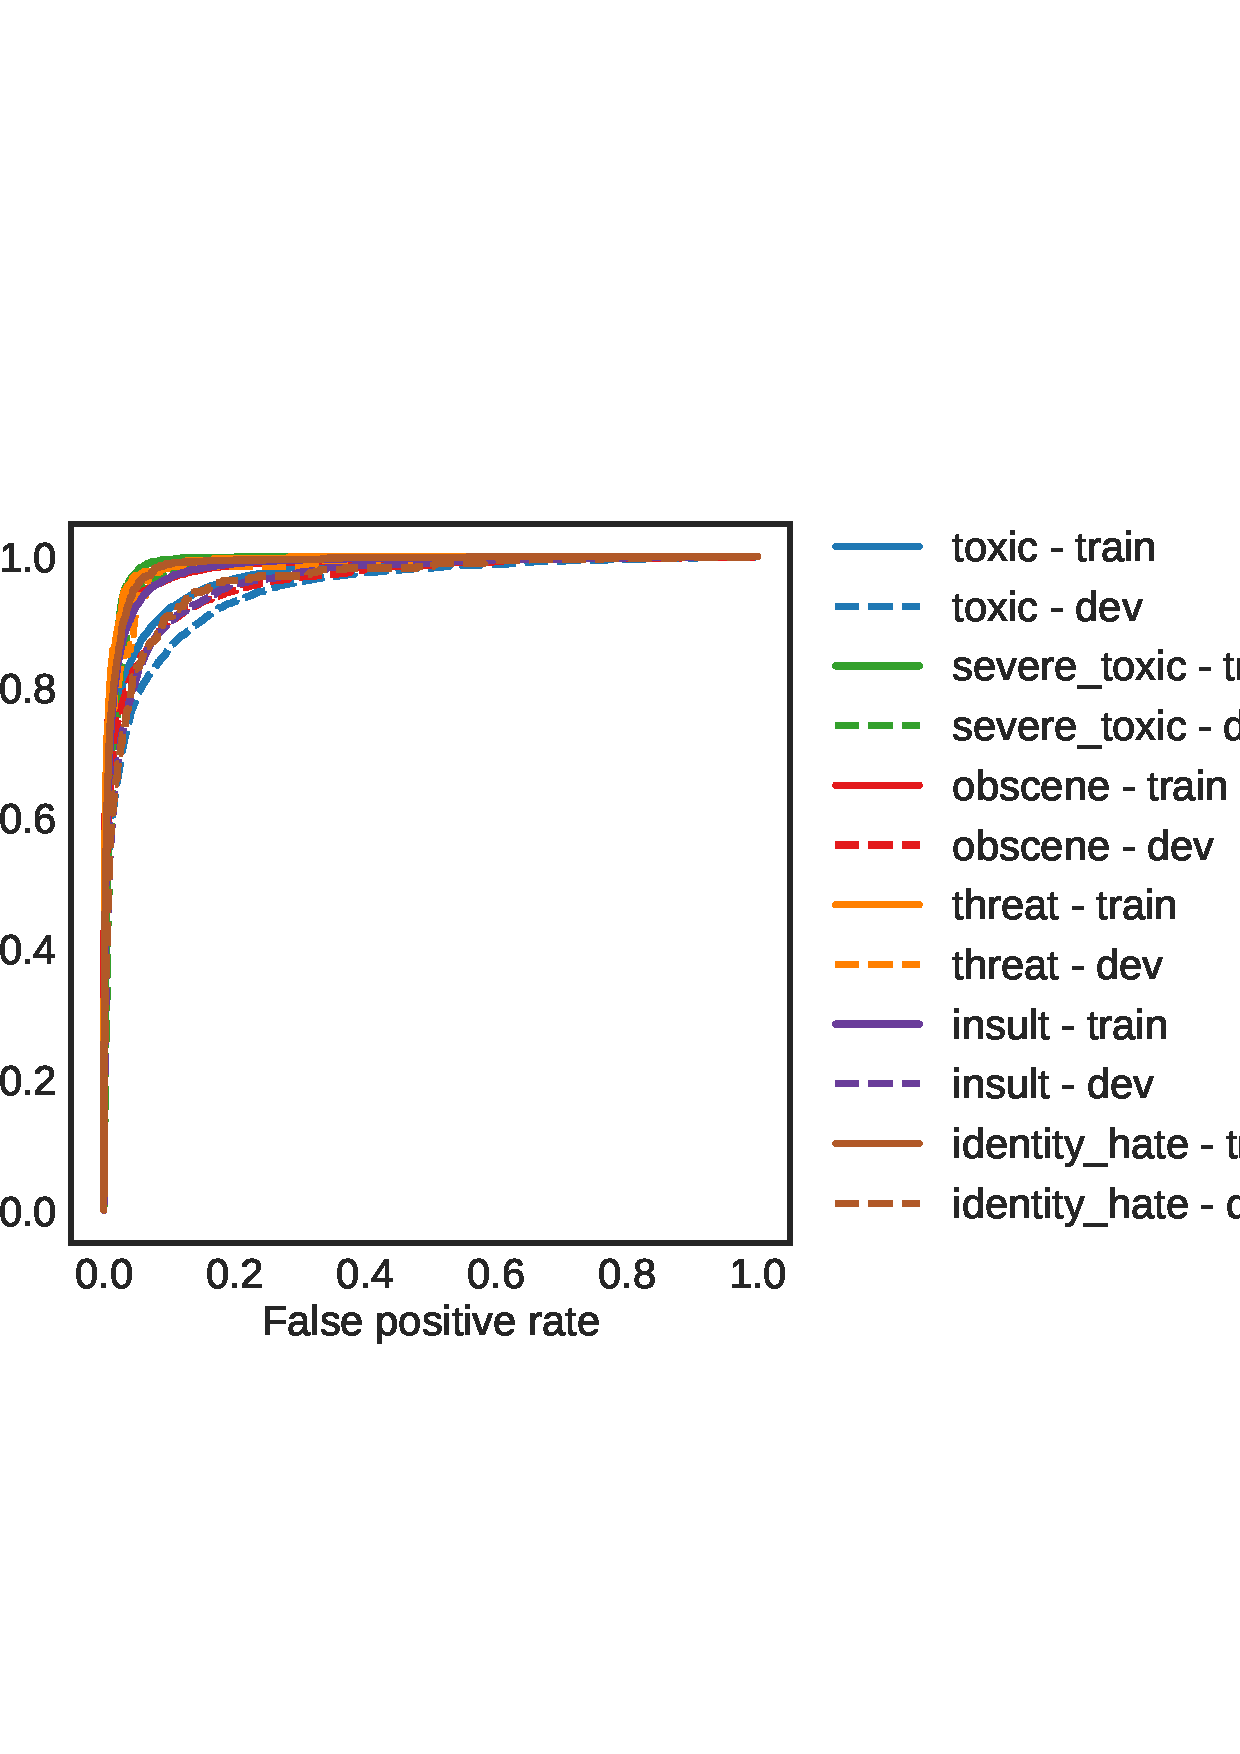
\includegraphics[width=4in]{ff_l3_h302010_f300_roc.png}
    \caption{The ROC curves for our baseline model's performance on each toxicity type.}
    \label{fig:roc}
    \end{figure}
   
   To investigate what factors are holding our baseline model back, we also plot the precision vs. recall performance of our classifier in Figure \ref{fig:prc}. Here we see that our performance may be more limited for the classes that have fewer training examples. We will need to account for this class imbalance going forward.
   
   \begin{figure}[h]
   \centering
   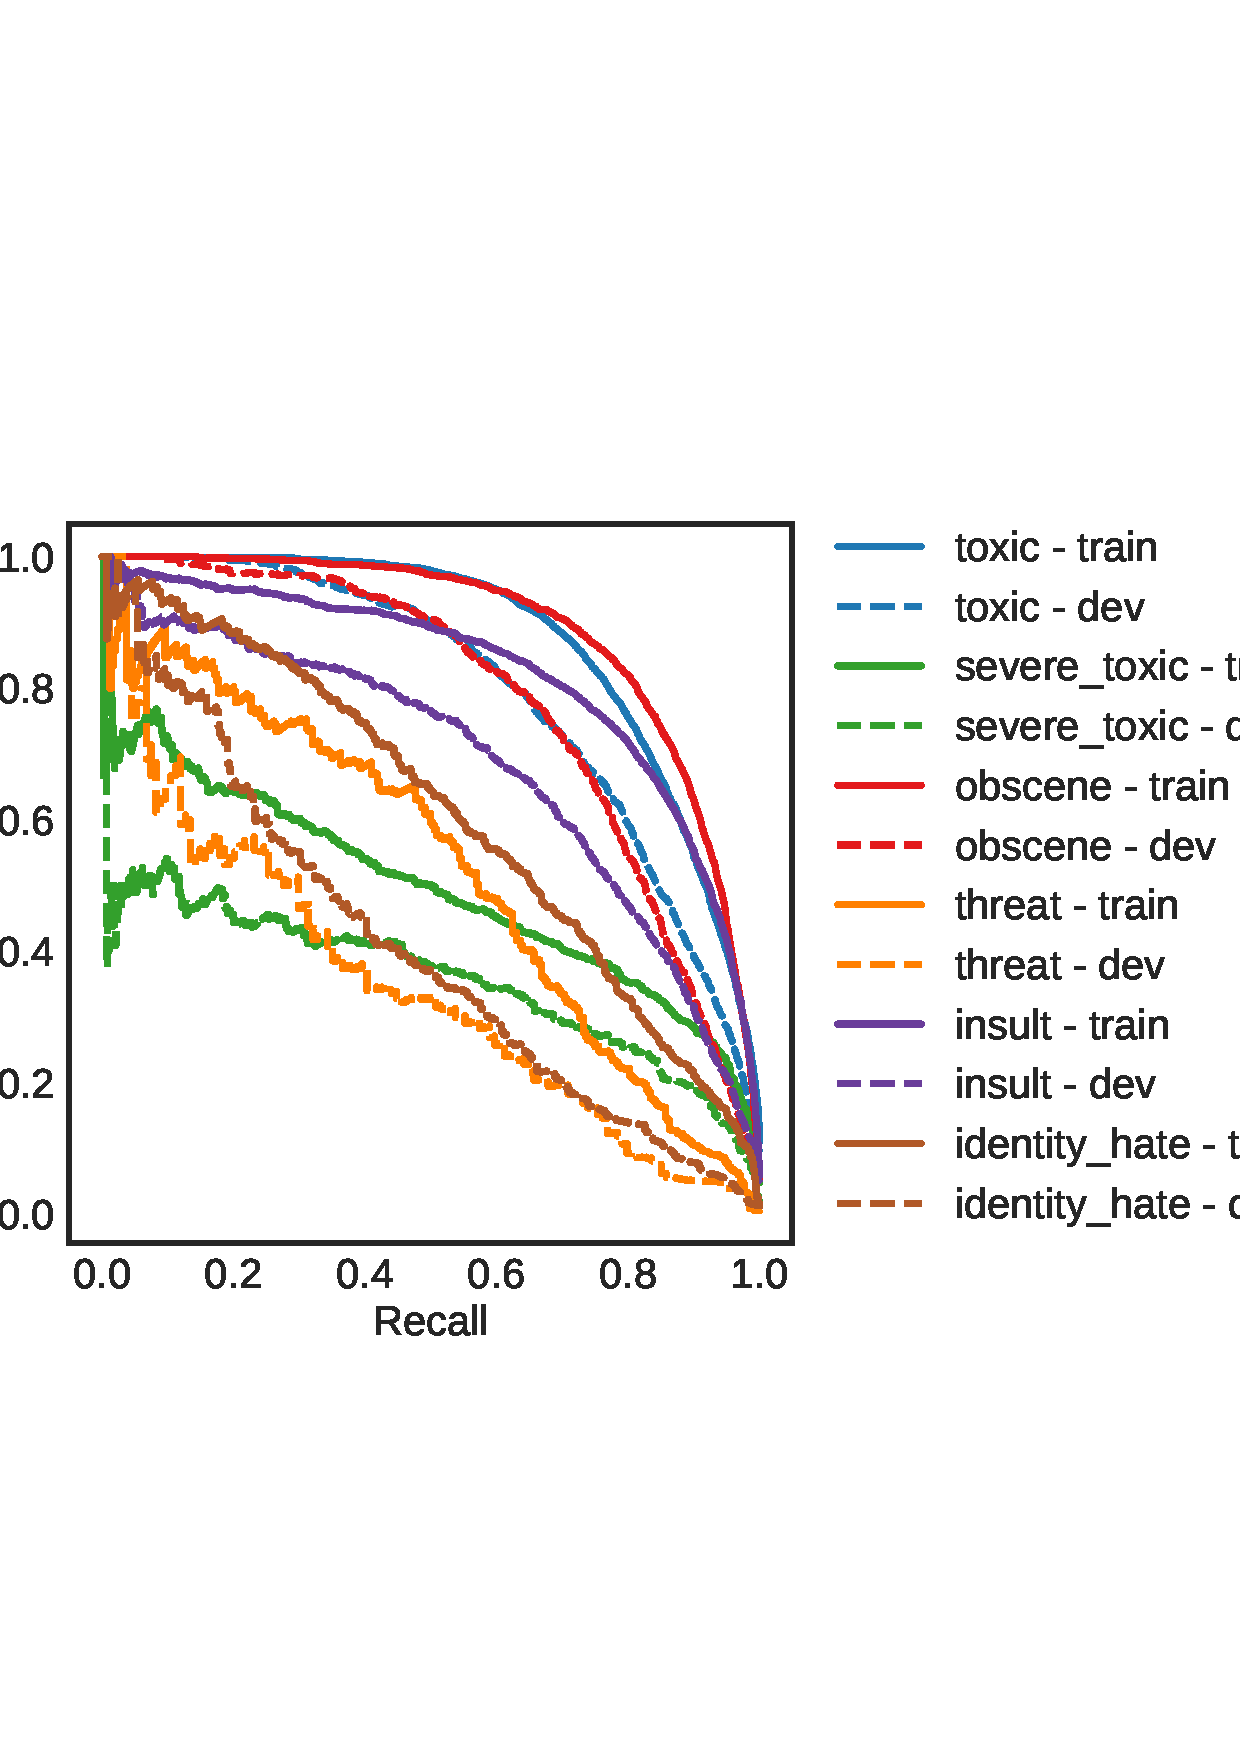
\includegraphics[width=4in]{ff_l3_h302010_f300_prc.png}
   \caption{The precision vs. recall performance for each toxicity type as classified by our baseline model.}
   \label{fig:prc}
   \end{figure}
   
    \item \textbf{Milestone Requirements:}
    \begin{enumerate}
      \item \textbf{Have collected all your data.} \checkmark
        \item \textbf{Have implemented a (very simple) baseline.} \checkmark
        \item \textbf{Have your evaluation pipeline set up.} \checkmark
        \item \textbf{Have run your baseline over your data and evaluated its performance} \checkmark
    \end{enumerate}
    
\end{enumerate}

\end{document}
